%&platex --translate-file=cp1250pl
\documentclass[times]{jtitauth}

\usepackage{url}
\usepackage{float}

\begin{document}

\title{Happiness Tracker\\}

\author{Alex Prut (master's degrees student in computer science) \\
University of Udine, Department of Mathematics and Computer Science \\ mail@alexprut.com}

\markboth{Alex Prut}
{Happiness Tracker}

\maketitle

\begin{abstract}
Happiness Tracker is a mobile application that allows you to track and increase your daily happiness.
The application is totally based on the emerging science of positive psychology. Therefore
the application will always communicate in a positive way directly and indirectly
both via words or visually (e.g. "I will never attend an anti-war rally; if you have a peace rally, invite me" — Mother Teresa).
More precisely the application bases its functionalities on the theory of labeling and gratitude.
Practically speaking the application asks you a fixed number of times during the day: "How do you feel?",
once a day it asks you to write something you are grateful for and finally
randomly during the day it shows you some motivational and
labeling phrases via notifications.
\end {abstract}

\begin{keywords}
positive psychology, mobile, gratitude, labeling theory, happiness, mood
\end{keywords}

* within the paper, with the assertion: \textit{(To be proved)} is meant that the phrase written right before the assertion is not been yet scientifically proved or is simply meant that it is a temporary not validated solution.

\section{Introduction}

\subsection{Goals and the science behind}
Happiness Tracker is a mobile application that allows you to track and try to increase your daily happiness.
The application is totally based on the emerging science of positive psychology \cite{1,2}. Therefore
the application will always communicate in a positive way directly and indirectly
both via words or visually (e.g. "I will never attend an anti-war rally; if you have a peace rally, invite me" — Mother Teresa).
More specifically if at average the mood of an user is "Sad", they will
continue to see warm colors, happy smiles and positive words.

To keep track of your overall daily happiness the application asks you daily a fixed
number of times via notifications: "How do you feel?" (the question phrase needs \textit{*To be proved}).
To express the actual happiness the user is able to choose between
3 different states: "Sad", "Normal" or "Happy" (see Fig.3).
The reason of only 3 different states if simply for it's simplicity, the user can express sadness,
a neutral state and finally a happy state (the number of the states needs \textit{*To be proved}).
The end user is also able to add an entry via the main page of the application (see Fig.1).
The application can show your average happiness for the last month, week and of the current day
(within the paper this feature is called and referenced as the \textbf{Mood tracker Feature}).

Furthermore, in order to increase your average happiness the application bases its functionalities
on two psychological theories such as the labeling theory \cite{3, 4, 5} and gratitude \cite{6, 7, 11}.

\begin{figure}[H]
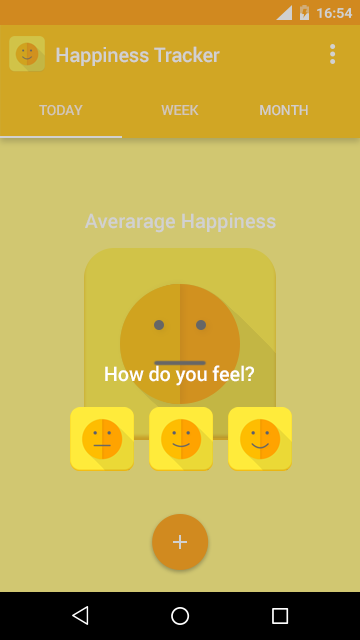
\includegraphics[scale=0.23]{HappinessTracker-notifications}
\label{fig:notifications}
\centering
\caption{Insertion of a new mood sample via the main page of the application}
\end{figure}

The labeling theory is how the self-identity and behavior of individuals may be determined
or influenced by the terms used to describe or classify them.
Practically the application implement the above theory by showing via
notifications some positive and labeling phrases
chosen randomly during the day (all the phrases needs \textit{*To be proved},
within the paper this feature is called and referenced as the \textbf{Labeling Feature}).

Lastly the experience of gratitude, which is a feeling or attitude in acknowledgment
of a benefit that one has received or will receive. 
Practically the application implement the above theory by daily asking once the end user to
write one thing for which he is grateful or was grateful during the day
(within the paper this feature is called and referenced as the \textbf{Gratitude Feature}).

\subsection{Design}
Colors and design is a very important aspect of the application, since it
can affect the mood of the end user and also the overall usage.
To express happiness warm colors are prefered and used, based on numerous researches the Yellow
color seems to be the color of happiness across the major cultures \cite{9} and in some researches was
classified by happy people as the color of happiness \cite{8}.
In order to communicate visually with the color of happiness, only monochromatic
shades of yellow are used (see the color palette in Fig. 2).
Since the first implementation of the application is on the Android platform the
color palette follows the Material Design \cite{10} color guidelines. 

\begin{figure}[H]
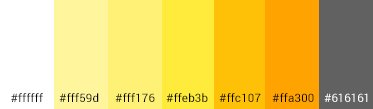
\includegraphics[width=\columnwidth]{HappinessTracker-color-palette}
\label{fig:color-palette}
\centering
\caption{Color Palette}
\end{figure}

To maintain the consistency of the application the same color palette is used for the state icons (see Fig. 3).

\begin{figure}[H]

\includegraphics[width=\columnwidth]{HappinessTracker-smile-icons}
\label{fig:smile-icons}
\centering
\caption{Mood states, smile icons}
\end{figure}

To express the 3 states of happiness the application uses different saturated shades
of yellow, respectively for the "Sad" state a less saturated yellow and for the
"Happy" state a more saturated yellow (see Fig. 4).

\begin{figure}[H]
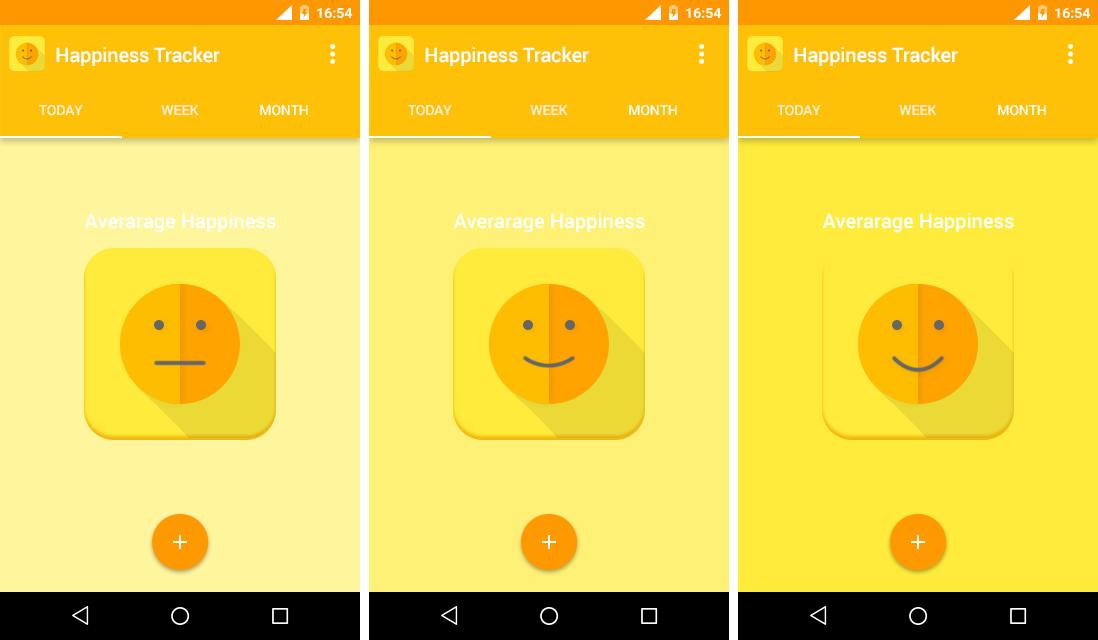
\includegraphics[width=\columnwidth]{HappinessTracker-happiness-types}
\label{fig:happiness-types}
\centering
\caption{Application design for the 3 different states of happiness}
\end{figure}

\section*{Conclusion}
The current MVP (Minimum Viable Product) implements only the Mood Tracker feature and the basic design.
Further work needs to be done in order to implement the Labeling Feature and the Gratitude Feature.
Besides all the *\textit{To be proved} assertions needs to be validate and proved scientifically.
So far a scientific method and measure was not adopted in order to validate the overall happiness of the 
end user in order to validate the utility and the efficacy of the application.
Even if not proved yet the expecting result is that with the use of the application the average happiness of the end user increase
indirectly.

\begin{thebibliography}{99}
\bibitem{1}Martin Seligman, ,,The new era of positive psychology'', {\it TED}, \url{http://www.ted.com/talks/martin_seligman_on_the_state_of_psychology}, 2014.
\bibitem{2}Wikipedia, ,,Positive psychology'', {\it Wikipedia}, \url{https://en.wikipedia.org/wiki/Positive_psychology}, extracted on July 2015.
\bibitem{3}Wikipedia, ,,Labeling Theory'', {\it Wikipedia}, \url{https://en.wikipedia.org/wiki/Labeling_theory}, extracted on July 2015.
\bibitem{4}Christopher J. Bryan, Gregory M. Walton, Todd Rogers and Carol S.Dweck, ,,Motivating voter turnout by invoking the self", \url{http://scholar.harvard.edu/files/todd_rogers/files/motivating.pdf}, 22 June 2011.
\bibitem{5}Alice M. Tybout, Richard F. Yalch,  ,,The Effect of Experience: A Matter of
Salience?", {\it Journal of Consumer Research}, \url{http://media.cbsm.com/uploads/1/TheEffectofExperience.pdf}, March 1980.
\bibitem{6}Wikipedia, ,,Gratitude'', {\it Wikipedia}, \url{https://en.wikipedia.org/wiki/Gratitude}, extracted on July 2015.
\bibitem{7}Alex M. Wood, Neil Stewart, John Maltby, P. Alex Linley,  ,,A Social–Cognitive Model of Trait and State Levels of Gratitude", {\it American Psychological Association}, \url{http://personalpages.manchester.ac.uk/staff/alex.wood/state\%20and\%20trait\%20gratitude.pdf}, 2007.
\bibitem{8}Helen R Carruthers, Julie Morris, Nicholas Tarrier and Peter J Whorwel, ,,The Manchester Color Wheel: development of a novel way of identifying color choice and its validation in healthy, anxious and depressed individuals", {\it MC Medical Research Methodology }, \url{http://www.biomedcentral.com/1471-2288/10/12}, 2010.
\bibitem{9}Mubeen M. Aslam, ,,Are you selling the right colour? A cross-cultural review of colour as a marketing cue", \url{http://ro.uow.edu.au/cgi/viewcontent.cgi?article=2092&context=commpapers}, 2005.
\bibitem{10}Google Inc., ,,Material Design Colors", \url{http://www.google.it/design/spec/style/color.html}, extracted on July 2015.
\bibitem{11}David Steindl-Rast, ,,Want to be happy? Be grateful'', {\it TED}, \url{http://www.ted.com/talks/david_steindl_rast_want_to_be_happy_be_grateful}, June 2013.
\end{thebibliography}

\end{document}